\documentclass[paperwidth=36in,paperheight=24in,landscape,fontscale=0.4,final]{baposter}
\usepackage[vlined]{algorithm2e}
\usepackage{times}
\usepackage{calc}
\usepackage{graphicx}
\usepackage{amsmath}
\usepackage{amssymb}
\usepackage{relsize}
\usepackage{multirow}
\usepackage{bm}

\usepackage{graphicx}
\usepackage{multicol}

\usepackage{pgfbaselayers}
\pgfdeclarelayer{background}
\pgfdeclarelayer{foreground}
\pgfsetlayers{background,main,foreground}

\usepackage{helvet}
%\usepackage{bookman}
\usepackage{palatino}

\newcommand{\captionfont}{\footnotesize}

\selectcolormodel{cmyk}

\graphicspath{{images/}}

%%%%%%%%%%%%%%%%%%%%%%%%%%%%%%%%%%%%%%%%%%%%%%%%%%%%%%%%%%%%%%%%%%%%%%%%%%%%%%%%
%%%% Some math symbols used in the text
%%%%%%%%%%%%%%%%%%%%%%%%%%%%%%%%%%%%%%%%%%%%%%%%%%%%%%%%%%%%%%%%%%%%%%%%%%%%%%%%
% Format 
\newcommand{\Matrix}[1]{\begin{bmatrix} #1 \end{bmatrix}}
\newcommand{\Vector}[1]{\Matrix{#1}}
\newcommand*{\SET}[1]  {\ensuremath{\mathcal{#1}}}
\newcommand*{\MAT}[1]  {\ensuremath{\mathbf{#1}}}
\newcommand*{\VEC}[1]  {\ensuremath{\bm{#1}}}
\newcommand*{\CONST}[1]{\ensuremath{\mathit{#1}}}
\newcommand*{\norm}[1]{\mathopen\| #1 \mathclose\|}% use instead of $\|x\|$
\newcommand*{\abs}[1]{\mathopen| #1 \mathclose|}% use instead of $\|x\|$
\newcommand*{\absLR}[1]{\left| #1 \right|}% use instead of $\|x\|$

\def\norm#1{\mathopen\| #1 \mathclose\|}% use instead of $\|x\|$
\newcommand{\normLR}[1]{\left\| #1 \right\|}% use instead of $\|x\|$

%%%%%%%%%%%%%%%%%%%%%%%%%%%%%%%%%%%%%%%%%%%%%%%%%%%%%%%%%%%%%%%%%%%%%%%%%%%%%%%%
% Multicol Settings
%%%%%%%%%%%%%%%%%%%%%%%%%%%%%%%%%%%%%%%%%%%%%%%%%%%%%%%%%%%%%%%%%%%%%%%%%%%%%%%%
\setlength{\columnsep}{0.7em}
\setlength{\columnseprule}{0mm}


%%%%%%%%%%%%%%%%%%%%%%%%%%%%%%%%%%%%%%%%%%%%%%%%%%%%%%%%%%%%%%%%%%%%%%%%%%%%%%%%
% Save space in lists. Use this after the opening of the list
%%%%%%%%%%%%%%%%%%%%%%%%%%%%%%%%%%%%%%%%%%%%%%%%%%%%%%%%%%%%%%%%%%%%%%%%%%%%%%%%
\newcommand{\compresslist}{%
\setlength{\sep}{0.5pt}%
\setlength{\parskip}{-0.5pt}%
\setlength{\parsep}{-0.5pt}%
}
\newtheorem{mydef}{Definition}

%%%%%%%%%%%%%%%%%%%%%%%%%%%%%%%%%%%%%%%%%%%%%%%%%%%%%%%%%%%%%%%%%%%%%%%%%%%%%%
%%% Begin of Document
%%%%%%%%%%%%%%%%%%%%%%%%%%%%%%%%%%%%%%%%%%%%%%%%%%%%%%%%%%%%%%%%%%%%%%%%%%%%%%

\begin{document}

%%%%%%%%%%%%%%%%%%%%%%%%%%%%%%%%%%%%%%%%%%%%%%%%%%%%%%%%%%%%%%%%%%%%%%%%%%%%%%
%%% Here starts the poster
%%%---------------------------------------------------------------------------
%%% Format it to your taste with the options
%%%%%%%%%%%%%%%%%%%%%%%%%%%%%%%%%%%%%%%%%%%%%%%%%%%%%%%%%%%%%%%%%%%%%%%%%%%%%%
\typeout{Poster Starts}
\background{
  \begin{tikzpicture}[remember picture,overlay]%
    \draw (current page.north west)+(-2em,-0em) node[anchor=north west] {\hspace{-2em}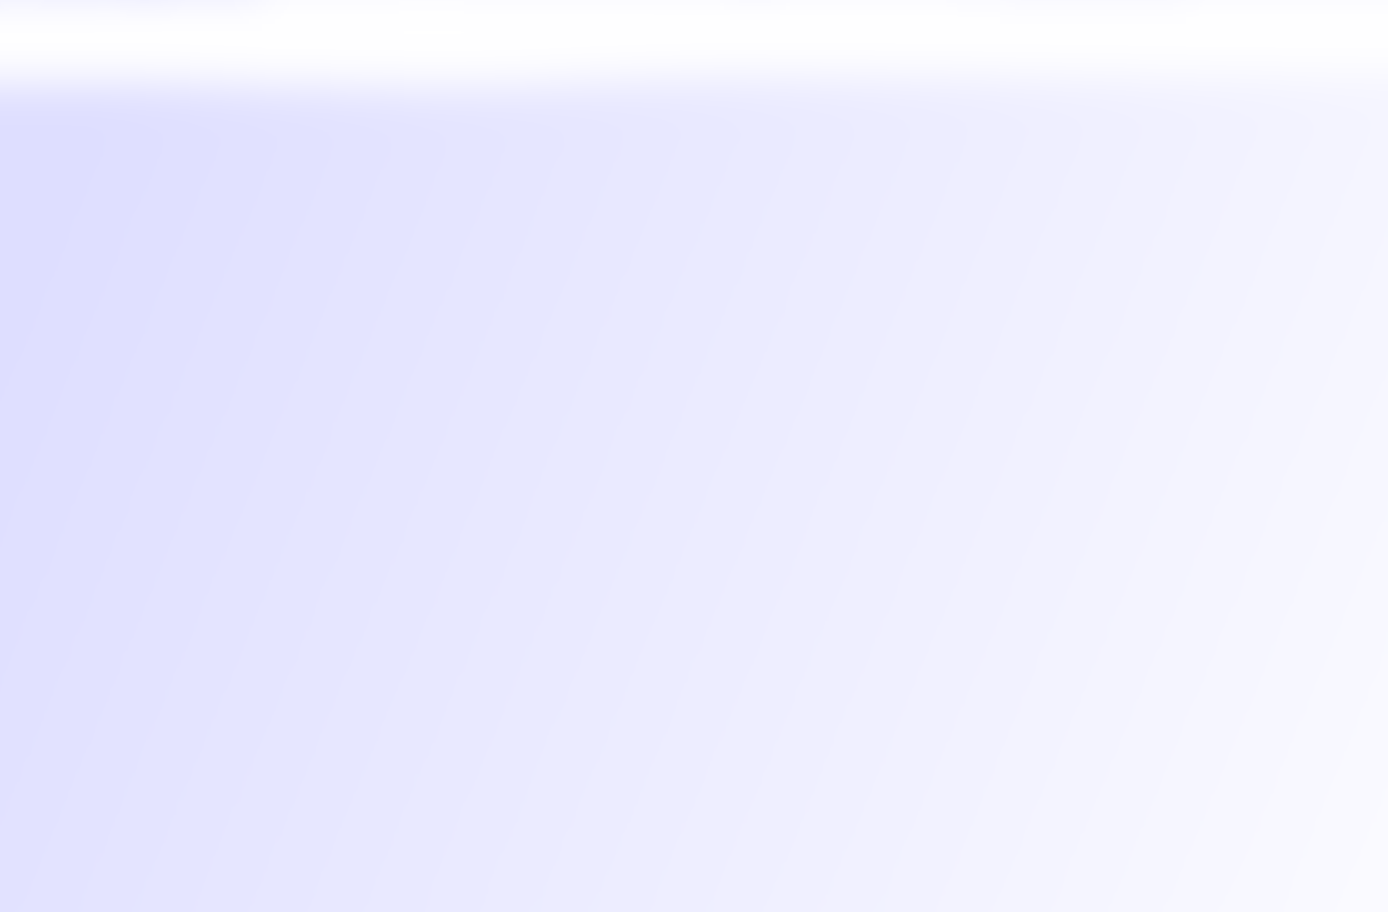
\includegraphics[height=1.1\textheight]{silhouettes_background}};
  \end{tikzpicture}%
}
\definecolor{silver}{cmyk}{0,0,0,0.3}
\definecolor{fsu_red}{cmyk}{0.0,0.72,0.62,0.47}
\definecolor{reddishyellow}{cmyk}{0,0.22,1.0,0.0}
\definecolor{black}{cmyk}{0,0,0.0,1.0}
\definecolor{darkYellow}{cmyk}{0,0,1.0,0.5}
\definecolor{darkSilver}{cmyk}{0,0,0,0.1}
\definecolor{gold}{cmyk}{0.06,0.14,0.39,0.08} %{0.00, 0.11, 0.45,0.07}
\definecolor{lightyellow}{cmyk}{0,0,0.3,0.0}
\definecolor{lighteryellow}{cmyk}{0,0,0.1,0.0}
\definecolor{lighteryellow}{cmyk}{0,0,0.1,0.0}
\definecolor{lightestyellow}{cmyk}{0,0,0.05,0.0}
\begin{poster}{
  % Show grid to help with alignment
  grid=false,
  % Column spacing
  colspacing=1em,
  % Color style
  bgColorOne=white,
  bgColorTwo=white,
  borderColor=fsu_red,
  headerColorOne=fsu_red,
  headerColorTwo=reddishyellow,
  headerFontColor=white,
  boxColorOne=gold,
  boxColorTwo=gold,
  % Format of textbox
  textborder=roundedleft,
  % Format of text header
  eyecatcher=false,
  headerborder=open,
  headerheight=0.08\textheight,
  headershape=roundedright,
  headershade=plain,
  headerfont=\Large\textsf, %Sans Serif
  boxshade=plain,
%  background=shade-tb,
  background=plain,
  linewidth=2pt
  }
  % Eye Catcher
  {} % No eye catcher for this poster. If an eye catcher is present, the title is centered between eye-catcher and logo.
  % Title
  {\sf %Sans Serif
  %\bf% Serif
  Boosting method for capturing high frequency limit order book dynamics}
  % Authors
  {\sf %Sans Serif
  % Serif
  Jian Wang\hspace{3em}
  jw09r@my.fsu.edu\hspace{3em}
  Florida State University
  }
  % University logo
  {{\begin{minipage}{16em}
    \hfill
    
\includegraphics[height=5.5em]{fsu_logo.pdf}
  \end{minipage}}
  }

  \tikzstyle{light shaded}=[top color=baposterBGtwo!30!white,bottom color=baposterBGone!30!white,shading=axis,shading angle=30]

  % Width of left inset image
     \newlength{\leftimgwidth}
     \setlength{\leftimgwidth}{0.78em+8.0em}

%%%%%%%%%%%%%%%%%%%%%%%%%%%%%%%%%%%%%%%%%%%%%%%%%%%%%%%%%%%%%%%%%%%%%%%%%%%%%%
%%% Now define the boxes that make up the poster
%%%---------------------------------------------------------------------------
%%% Each box has a name and can be placed absolutely or relatively.
%%% The only inconvenience is that you can only specify a relative position 
%%% towards an already declared box. So if you have a box attached to the 
%%% bottom, one to the top and a third one which should be in between, you 
%%% have to specify the top and bottom boxes before you specify the middle 
%%% box.
%%%%%%%%%%%%%%%%%%%%%%%%%%%%%%%%%%%%%%%%%%%%%%%%%%%%%%%%%%%%%%%%%%%%%%%%%%%%%%
    %
    % A coloured circle useful as a bullet with an adjustably strong filling
    \newcommand{\colouredcircle}[1]{%
      \tikz{\useasboundingbox (-0.2em,-0.32em) rectangle(0.2em,0.32em); \draw[draw=black,fill=baposterBGone!80!black!#1!white,line width=0.03em] (0,0) circle(0.18em);}}

%%%%%%%%%%%%%%%%%%%%%%%%%%%%%%%%%%%%%%%%%%%%%%%%%%%%%%%%%%%%%%%%%%%%%%%%%%%%%%
  \headerbox{\textbf{Contribution}}{name=contribution,column=0,row=0}{
%%%%%%%%%%%%%%%%%%%%%%%%%%%%%%%%%%%%%%%%%%%%%%%%%%%%%%%%%%%%%%%%%%%%%%%%%%%%%%
 More than half of the markets in today's fast-paced financial world now use a limit order book(LOB) to facilitate trade(Rosu 2009). Therefore, capturing the dynamics of high frequency LOBs become a challenging task for our financial engineering researchers. We propose boosting machine learning methods to predict future spread crossing opportunities. Our main contributions are concluded as follows:
 \begin{itemize}
 \item Use boosting methods to improve the performance for weaker classifier.
 \item Predict the future spread crossing opportunities based on fixed time interval.
 \item Compare the accuracy rate and computation time among different machine learning methods
 \end{itemize}
 }

%%%%%%%%%%%%%%%%%%%%%%%%%%%%%%%%%%%%%%%%%%%%%%%%%%%%%%%%%%%%%%%%%%%%%%%%%%%%%%
  \headerbox{\textbf{Definition}}{name=model,column=0,below=contribution,above=bottom}{
%%%%%%%%%%%%%%%%%%%%%%%%%%%%%%%%%%%%%%%%%%%%%%%%%%%%%%%%%%%%%%%%%%%%%%%%%%%%%%
\begin{mydef}
An order $x=(p_x, \omega_x,t_x)$ submitted at time $t_x$ with price $p_x$ and size 
$\omega_x>0$ (respectively, $\omega_x<0$) is a commitment to sell (respectively,buy) up to $|\omega_x|$ units of the traded asset at a price no less than (respectively, no greater than) $p_x$.
\end{mydef}
\begin{mydef}
An LOB $\mathcal{L}(t)$ is the set of all active orders in a market at time t.
\end{mydef}
\begin{mydef}
The bid price at time t is the highest stated price among active buy orders at time t,
\begin{align*}
      b(t):=\max_{x \in \mathcal{B}(t)} p_x
\end{align*}
The ask price at time t is the lowest stated price among active sell orders at time t,
\begin{align*}
      a(t):=\min_{x \in \mathcal{A}(t)} p_x
\end{align*}
\end{mydef}
\begin{mydef}
The bid-ask spread at time t is $s(t):=a(t)-b(t)$.
The mid price at time t is $m(t):= [a(t)+b(t)]/2$
\end{mydef}
\begin{mydef}
Bid higher spread crossing at time t after $\Delta t$ time interval is $P_{t+\Delta t}^{Bid}>P_{t}^{Ask}$, ask lower spread crossing at time t after $\Delta t$ time interval is $P_{t+\Delta t}^{Ask}<P_{t}^{Bid}$, no spread crossing at time t after $\Delta t$ time interval is $P_{t+\Delta t}^{Bid}<=P_{t}^{Ask}$ and $P_{t+\Delta t}^{Ask}>=P_{t}^{Bid}$
\end{mydef}
  }


%%%%%%%%%%%%%%%%%%%%%%%%%%%%%%%%%%%%%%%%%%%%%%%%%%%%%%%%%%%%%%%%%%%%%%%%%%%%%%
  \headerbox{\textbf{Data Set}}{name=dataset,column=1,row=0}{
%%%%%%%%%%%%%%%%%%%%%%%%%%%%%%%%%%%%%%%%%%%%%%%%%%%%%%%%%%%%%%%%%%%%%%%%%%%%%% 
Our dataset contains limit order prices on 2012-06-21 of four stocks from NASDAQ (Apple,Amazon,Intel and Microsoft). For each stock, it divided into two major components: the message book and the order book. 
 \begin{itemize}
 \item Message book: contains time when the order book came, prices,volumes, event types and directions.
 \item Order book: contains price levels, prices and volumes in each level for every event.
 \end{itemize}
Time is in sec and minimum time change is nanosecond. Price is in dollar
and each tick is one cent. 7 Event types, such as execution, cancellation and so
on. 2 Directions, ask and bid.

 
 
  }
%%%%%%%%%%%%%%%%%%%%%%%%%%%%%%%%%%%%%%%%%%%%%%%%%%%%%%%%%%%%%%%%%%%%%%%%%%%%%%
  \headerbox{\textbf{Snapshots of LOBS}}{name=snapshots,column=1,below=dataset,span=1}{
%%%%%%%%%%%%%%%%%%%%%%%%%%%%%%%%%%%%%%%%%%%%%%%%%%%%%%%%%%%%%%%%%%%%%%%%%%%%%%
  \begin{tabular}{ll}
    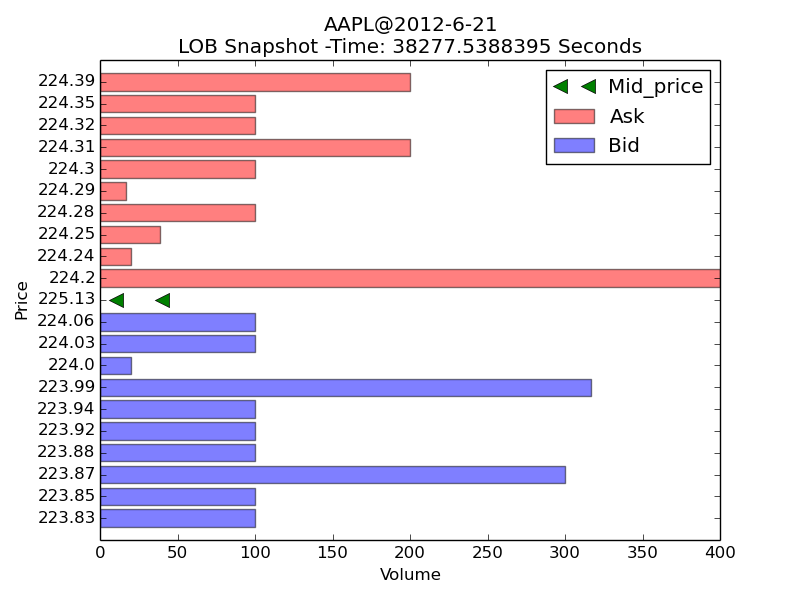
\includegraphics[width=0.45\linewidth,height=0.4\linewidth]{AAPL_snapshot}&
    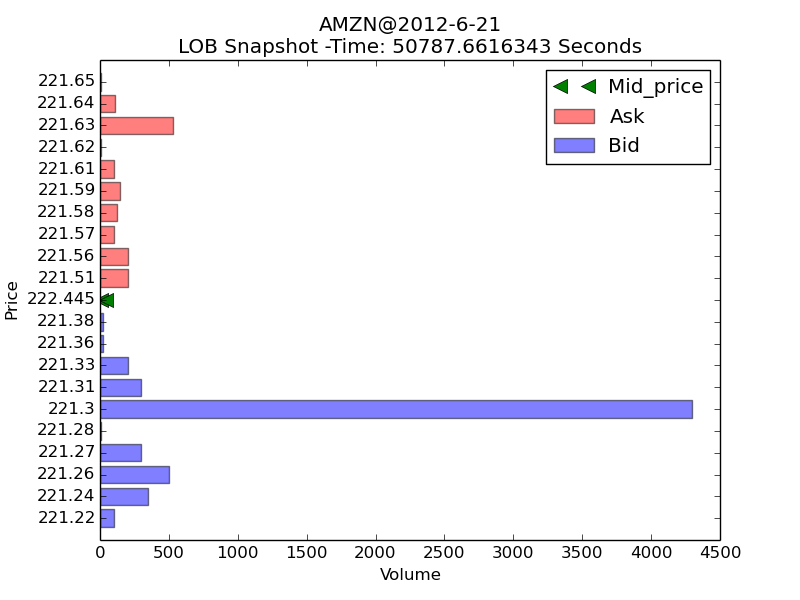
\includegraphics[width=0.45\linewidth,height=0.4\linewidth]{AMZN_snapshot}\\
    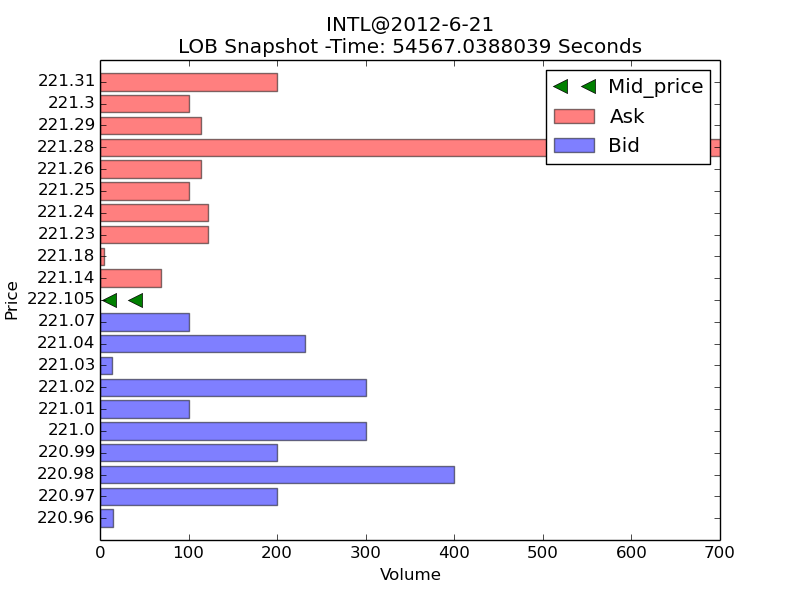
\includegraphics[width=0.45\linewidth,height=0.4\linewidth]{INTL_snapshot}&
    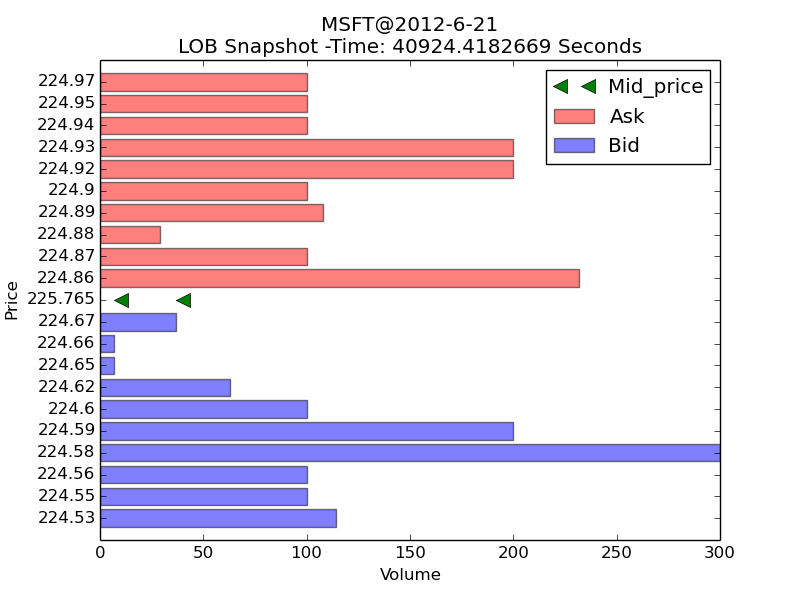
\includegraphics[width=0.45\linewidth,height=0.4\linewidth]{MSFT_snapshot}   
  \end{tabular}
\textbf{Figure 1} shows the snapshot of 10 level ask and bid prices of four stocks. The red bars show the ask prices, the blue bars represent the bid prices and the green triangle is the mid price.
  }
   \headerbox{\textbf{Conclusion and future works}}{name=conclusion,column=1,row=0,span=1,above=bottom,below=snapshots}{
      %%%%%%%%%%%%%%%%%%%%%%%%%%%%%%%%%%%%%%%%%%%%%%%%%%%%%%%%%%%%%%%%%%%%%%%%%%%%%%

{1.Boosting methods performance better than other machine learning models in this case}\\
{2.Can use high performance method such as parallel computing to improve the speed}\\
{3.Can test the Profit and Loss(PNL) which traders mainly concern}\\

        }%
%%%%%%%%%%%%%%%%%%%%%%%%%%%%%%%%%%%%%%%%%%%%%%%%%%%%%%%%%%%%%%%%%%%%%%%%%%%%%%
  \headerbox{\textbf{Boosting methods}}{name=boosting,column=2,span=2,row=0}{
%%%%%%%%%%%%%%%%%%%%%%%%%%%%%%%%%%%%%%%%%%%%%%%%%%%%%%%%%%%%%%%%%%%%%%%%%%%%%%

        Boosting method is a procedure that combines the outputs of many "weak" classifiers to produce a powerful "committee", it was originally designed for classification problems and later extended to regression.

  }%
  \headerbox{\textbf{AdaBoost}}{name=adaBoost,column=2,below=boosting}{
%%%%%%%%%%%%%%%%%%%%%%%%%%%%%%%%%%%%%%%%%%%%%%%%%%%%%%%%%%%%%%%%%%%%%%%%%%%%%%

        AdaBoost, formulated by Yoav Freund and Robert Schapire, is the most popular boosting algorithm, it puts more weights on the false
        classification data:\\
        \textbf{Algorithm:} \\      
		\begin{algorithm}[H]
		    \dontprintsemicolon
		    \linesnumbered
		    \nl Initialize the observation weights $\omega_i$=$1/N$,$i$=1,2,...,$N$\;
		    \nl \For{m=1 to M}{
		      Fit a classifer $G_m(x)$ to the training data using weights $\omega_i$\;
		       Compute \\
		      \begin{equation*}
		      err_m=\frac{\sum_{i=1}^{N}\omega_i I(y_i \neq G_m(x_i))}{\sum_{i=1}^{N}\omega_i}
		      \end{equation*}
		     Compute $\alpha_m=log((1-err_m)/err_m)$\;
		     Set $\omega_i \gets \omega_i \cdot exp[\alpha_m \cdot I(y_i \neq G_m(x_i))]$, $i =1,2,...,N$ \;
		    }
		    \nl Output $G(x)=sign[\sum_{m=1}^{M}\alpha_m G_m(x)]$ 
		  \end{algorithm}
  }%  
    \headerbox{\textbf{Gradient boosting}}{name=Gradient boosting,column=3,below=boosting}{
  %%%%%%%%%%%%%%%%%%%%%%%%%%%%%%%%%%%%%%%%%%%%%%%%%%%%%%%%%%%%%%%%%%%%%%%%%%%%%%
  
          Gradient boosting uses gradient descent methods to
          minimize the residual in each step:\\
          \textbf{Algorithm:}\\         
         \begin{algorithm}[H]
         		    \dontprintsemicolon
         		    \linesnumbered
         		    \nl Initialize $f_0(x)=argmin_\gamma \sum_{i=1}^NL(y_i,\gamma)$\;
         		    \nl \For{m=1 to M}{
         		    \For{i=1,2,...,N}
         		    {\begin{equation*}
         		    r_{im}=-[\frac{\partial L(y_i,f(x_i))}{\partial f(x_i)}]_{f=f_{m-1}}
         		             		    \end{equation*}
         		             		    }

         		     Fit a regression tree to the targets $r_{im}$ giving terminal regions $R_{jm}$, $j$=1,2,...,$J_m$\;
         		     \For{j=1,2,...,$J_m$}
         		    {
         		    $$\gamma_{jm}=arg\min_\gamma \sum_{x_i\in R_{jm}} L(y_i,f_{m-1}(x_i)+\gamma)$	
         		    }
         		    Update $f_m(x) =f_{m-1}(x)+\sum_{j=1}^{J_m}\gamma_{jm}I(x \in R_{jm})$\;
         		    }
         		    \nl Output $\hat{f}(x)=f_M(x)$ 
         		  \end{algorithm} 
  



    }
%%%%%%%%%%%%%%%%%%%%%%%%%%%%%%%%%%%%%%%%%%%%%%%%%%%%%%%%%%%%%%%%%%%%%%%%%%%%%%
  \headerbox{\textbf{Numerical results for AAPL}}{name=resultsAAPL,column=2,span=1,below=adaBoost}{
%%%%%%%%%%%%%%%%%%%%%%%%%%%%%%%%%%%%%%%%%%%%%%%%%%%%%%%%%%%%%%%%%%%%%%%%%%%%%%
\small{We try to predict the future 5 seconds spread crossing situation. Training samples are 8000 and test samples 2000. The parameter for adaboosting and gradient boosting are: depth =3 and iterations =500. Computer is 8G memory
and Intel Xeon E3 processor(4 cores), the results are listed in the following table}\\

\small{
\begin{tabular}{|l|l|l|}
\hline
   Methods & Accuracy rate & CPU time \\
   \hline
   Logistic & 57.15\% & 0.06\\
   Ridge(alpha=1)& 59.83\% & 0.01\\
   Lasso(alpha=0.001)& 60.75\%&16.54\\
   SVM& 60.15\%& 4.04\\
   Decision tree& 51.40\%&    0.24\\
   Ada Boosting Tree& {\color{red}{72.90\%}}&30.19\\
   Gradient Boosting Tree& \color{red}{71.95\%}& 14.53\\
   \hline   
   \end{tabular} }
   
\textbf{Table 1} \small{shows the predicting accuracy and computation time for AAPL data under different machine learning methods.}

  }%
  
   \headerbox{\textbf{Numerical results for AMZN}}{name=resultsAMZN,column=3,span=1,below=Gradient boosting}{
  %%%%%%%%%%%%%%%%%%%%%%%%%%%%%%%%%%%%%%%%%%%%%%%%%%%%%%%%%%%%%%%%%%%%%%%%%%%%%%
  We applied the same parameters that used in AAPL to test AMZM data\\
  

  \begin{tabular}{|l|l|l|}
  \hline
     Methods & Accuracy rate & CPU time \\
     \hline
     Logistic &66.97\%&      1.75\\
     Ridge(alpha=1)&      64.32\%&      0.01\\
     Lasso(alpha=0.001)&      65.60\%&      16.60\\
     SVM&      64.54\%   &   6.19\\
     Decision tree&  56.01\%& 0.26\\
     Ada Boosting Tree& \color{red}{74.03\%} &29.40\\
    Gradient Boosting Tree & \color{red} {77.23\%} &  14.4\\


     \hline   
     \end{tabular} 
     
 \textbf{Table 2} \small{shows the predicting accuracy and computation time for AMZM data under different machine learning methods. We can also see that the performances for AMZN are better than for AAPL to some extent. }
  
  
    }%
    
    
%%%%%%%%%%%%%%%%%%%%%%%%%%%%%%%%%%%%%%%%%%%%%%%%%%%%%%%%%%%%%%%%%%%%%%%%%%%%%%%
%  \headerbox{\textbf{Funding}}{name=funding,column=3,span=1,above=bottom}{
%%%%%%%%%%%%%%%%%%%%%%%%%%%%%%%%%%%%%%%%%%%%%%%%%%%%%%%%%%%%%%%%%%%%%%%%%%%%%%%
%  \smaller 
%  This work was supported in part by Microsoft Research through the European PhD Scholarship Programme.
%  }%
%%%%%%%%%%%%%%%%%%%%%%%%%%%%%%%%%%%%%%%%%%%%%%%%%%%%%%%%%%%%%%%%%%%%%%%%%%%%%%
  \headerbox{\textbf{References}}{name=references,column=2,span=2,above=bottom,below=resultsAAPL}{
%%%%%%%%%%%%%%%%%%%%%%%%%%%%%%%%%%%%%%%%%%%%%%%%%%%%%%%%%%%%%%%%%%%%%%%%%%%%%%
    \scriptsize
    \vspace{-1em}
    \bibliographystyle{ieee}
    \renewcommand{\section}[2]{\vskip 0.03em}
      \begin{thebibliography}{1}\itemsep=-0.4em
      \setlength{\baselineskip}{0.2em}
     
           \bibitem{alec:model}
             Alec N.Kercheval,Yuan Zhang        
             \newblock Modeling high-frequency limit order book dynamics
             with support vector machines        
             \newblock In {\em Quantitative finance 2014}
     
      \bibitem{rosu:dynamic}
      Rosu,I., 
      \newblock A dynamic model of the limit order book. 
      \newblock In {\em Rev.Financ.Stud.,2009,22,4601-4641.}
      
        \bibitem{:recognition}
                Trevor Hastie, Robert Tibshirani, Jerome Friedman      
                \newblock The Elements of Statistical Learning: Data Mining, Inference, and Prediction,Second Edition        
               
      \end{thebibliography}
  }%
  
  

\end{poster}%
%
\end{document}
